\chapter{Results}\label{chapter_4}

The following Figure~\ref{fig:spider_resnet50} shows the best macro-averaged f1-score per pre-training domain achieved with a Resnet50 model. 
The semi-transparent area indicates the sample standard deviation.

\begin{figure}[H]
    \begin{center}
    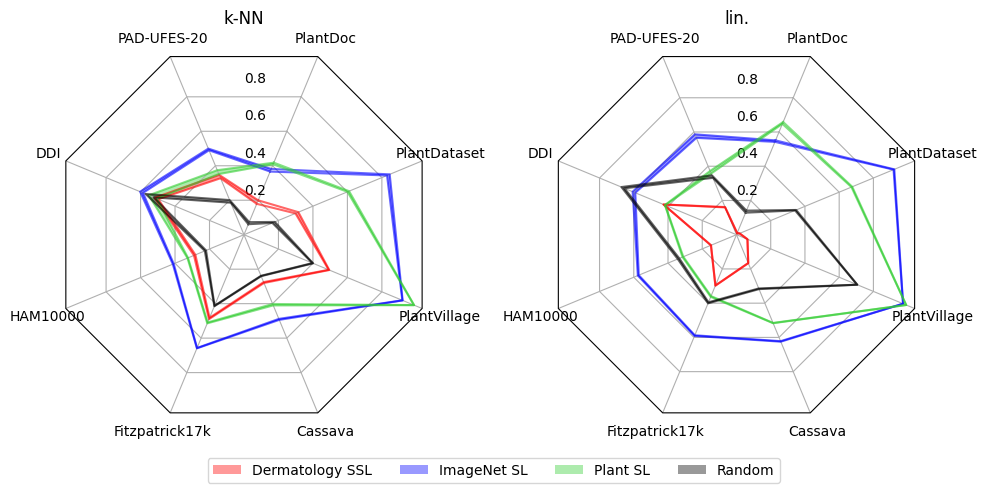
\includegraphics[width=15cm]{spider_resnet50.png}
    \caption{Linear evaluation scores of Resnet50}\label{fig:spider_resnet50}
    \end{center}
\end{figure}

Overall the ImageNet based approach outperforms the other approaches in most cases.
PlantDoc and the \gls{pvd} are only tasks in which the plant based model actually get the best result.
The dermatology based model performs very poorly and gets beaten by the ramdomly initialized model in some multiple cases.
The scores are never significantly better than the other pre-trained models. 
% The model which was trained on ImageNet with \gls{ssl} was not put into the graphic, but the tables show that these scores are bad as well. 
This indicates a problem with the type of training rather than with the data per se.

The respective results of \gls{vit} models can bee seen in Figure~\ref{fig:spider_vit_t16}.

\begin{figure}[H]
    \begin{center}
    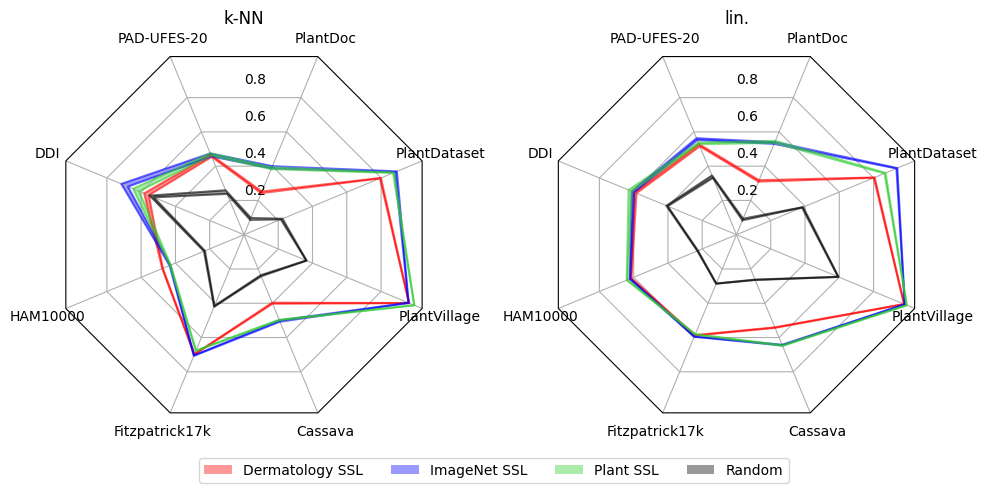
\includegraphics[width=15cm]{spider_vit_t16.png}
    \caption{Linear evaluation of \gls{vit}}\label{fig:spider_vit_t16}
    \end{center}
\end{figure}

The scores look similar. 
The scores of the plant based model are better in some tasks than the model trained with \gls{sl} on ImageNet, but not better than the \gls{ssl} variant. 
All DINO based models are relatively close to each other. 
This is probably due to their way of training rather than the data.

\subsection{Results on plant disease tasks}

All f1-scores are listed in Table~\ref{tab:f1_scores_resnet_plant} for Resnet50 and Table~\ref{tab:f1_scores_vit_plant} for \gls{vit} respectively.

\begin{table}[H]
    \centering
    \caption{F1-scores of ResNet50 on plant downstream tasks\label{tab:f1_scores_resnet_plant}}
    {\fontsize{8pt}{10pt}\selectfont 
    \csvreader[tabular=|l|c|c|c|c|c|c|c|c|,
    filter expr={test{\ifnumgreater{\thecsvinputline}{3}}},
    table head=\hline\multicolumn{1}{|c|}{} & \multicolumn{2}{c|}{\bfseries PlantDoc} & \multicolumn{2}{c|}{\bfseries PlantDataset} & \multicolumn{2}{c|}{\bfseries Cassava} & \multicolumn{2}{c|}{\bfseries PlantVillage}\\\hline Pre-training & Lin. & k-NN & Lin. & k-NN & Lin. & k-NN & Lin. & k-NN \\\hline,
    table foot=\hline\multicolumn{1}{|c|}{ZeroR baseline} & \multicolumn{2}{c|}{0.3} & \multicolumn{2}{c|}{1.8} & \multicolumn{2}{c|}{15.2} & \multicolumn{2}{c|}{0.5}\\\hline]{../../results/f1_scores_resnet_plant.csv}{}%
    {\csvcoli\ & \csvcolii & \csvcoliii & \csvcoliv & \csvcolv & \csvcolvi & \csvcolvii & \csvcolviii & \csvcolix}%
    }
\end{table}

\subsection{Vision Transformers}

% \subsection{Resnet}

% \subsection{Vision Transformers}





The
while Table~\ref{tab:f1_scores_resnet_derma} and .
Table~\ref{tab:f1_scores_vit_derma} and . 


In the linear evaluation the plant based model is actually a bit better than the ImageNet based model, but with \gls{knn} the difference becomes negligible.



% \subsection{Linear evaluation on features}
% \section{Overview}

\begin{table}[H]
    \centering
    \caption{F1-scores of ResNet50 on dermatology downstream tasks\label{tab:f1_scores_resnet_derma}}
    {\fontsize{8pt}{10pt}\selectfont 
    \csvreader[tabular=|l|c|c|c|c|c|c|c|c|,
    filter expr={test{\ifnumgreater{\thecsvinputline}{3}}},
    table head=\hline\multicolumn{1}{|c|}{} & \multicolumn{2}{c|}{\bfseries DDI} & \multicolumn{2}{c|}{\bfseries PAD-UFES-20} & \multicolumn{2}{c|}{\bfseries HAM10000} & \multicolumn{2}{c|}{\bfseries Fitzpatrick17k}\\\hline Pre-training & Lin. & k-NN & Lin. & k-NN & Lin. & k-NN & Lin. & k-NN \\\hline,
    table foot=\hline\multicolumn{1}{|c|}{ZeroR baseline} & \multicolumn{2}{c|}{42.6} & \multicolumn{2}{c|}{8.9} & \multicolumn{2}{c|}{10.7} & \multicolumn{2}{c|}{28.1}\\\hline]{../../results/f1_scores_resnet_derma.csv}{}%
    {\csvcoli\ & \csvcolii & \csvcoliii & \csvcoliv & \csvcolv & \csvcolvi & \csvcolvii & \csvcolviii & \csvcolix}%
    }
\end{table}











\section{Subsampling}
% NOTE: order by size
\subsection{PlantDoc}

\begin{figure}[H]
    \begin{center}
    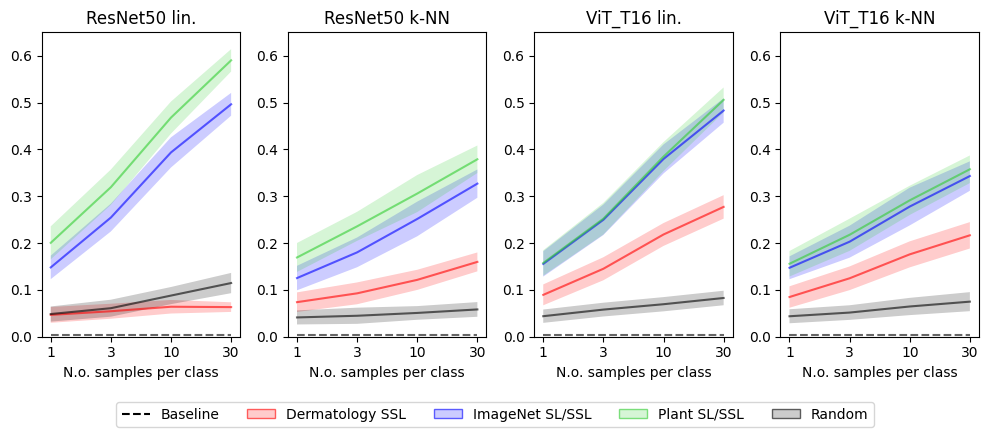
\includegraphics[width=15cm]{lines_plantdoc.png}
    \caption{Results of linear evaluation on subsampled sets from PlantDoc}\label{fig:lines_plantdoc}
    \end{center}
\end{figure}

\subsection{PlantDataset}

\begin{figure}[H]
    \begin{center}
    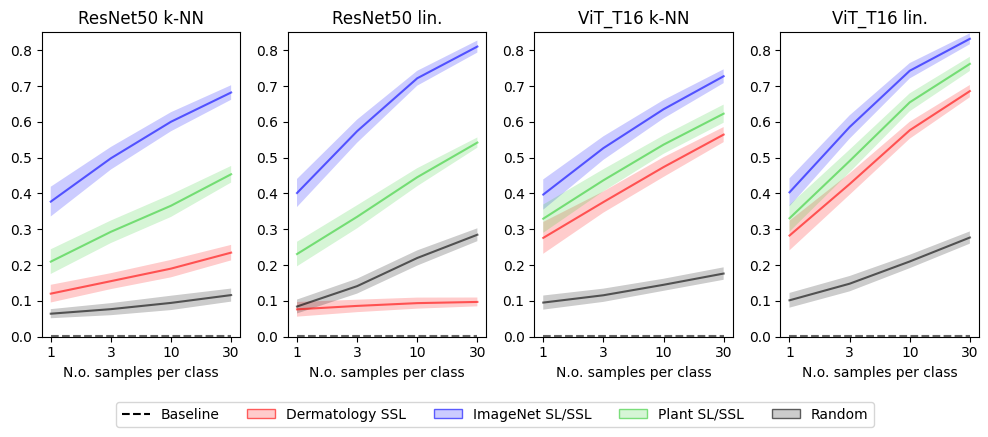
\includegraphics[width=15cm]{lines_plantdataset.png}
    \caption{Results of linear evaluation on subsampled sets from PlantDataset}\label{fig:lines_plantdataset}
    \end{center}
\end{figure}

\subsection{Cassava Leaf Disease Classification}

\begin{figure}[H]
    \begin{center}
    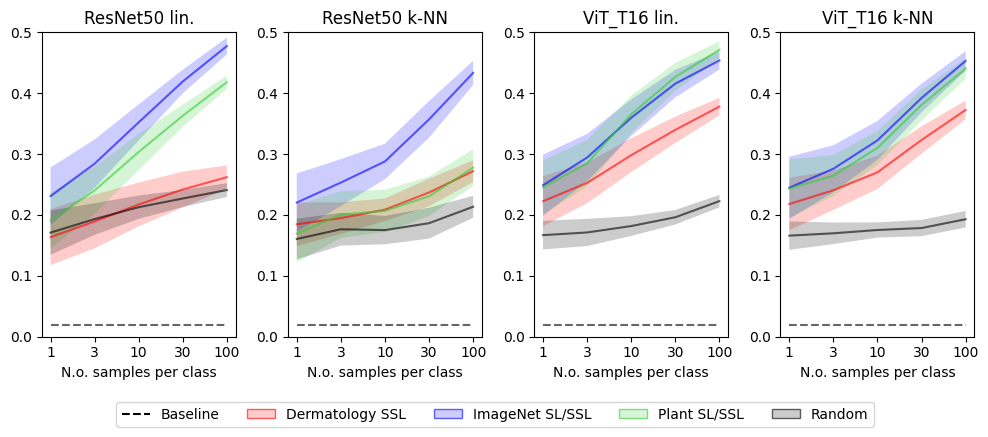
\includegraphics[width=15cm]{lines_cassava.png}
    \caption{Results of linear evaluation on subsampled sets from Cassava}\label{fig:lines_cassava}
    \end{center}
\end{figure}

\subsection{PlantVillage Dataset (PVD)}

\begin{figure}[H]
    \begin{center}
    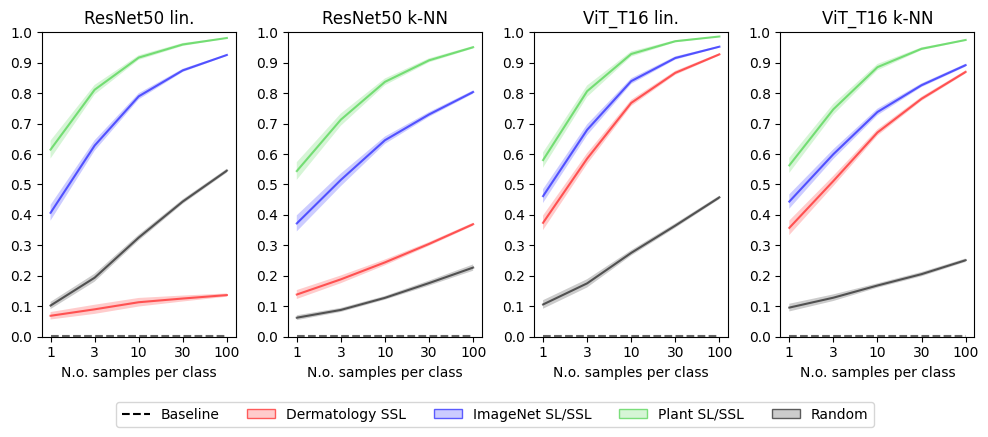
\includegraphics[width=15cm]{lines_plantvillage.png}
    \caption{Results of linear evaluation on subsampled sets from \gls{pvd}}\label{fig:lines_plantvillage}
    \end{center}
\end{figure}

\subsection{Diverse Dermatology Images (DDI)}

\begin{figure}[H]
    \begin{center}
    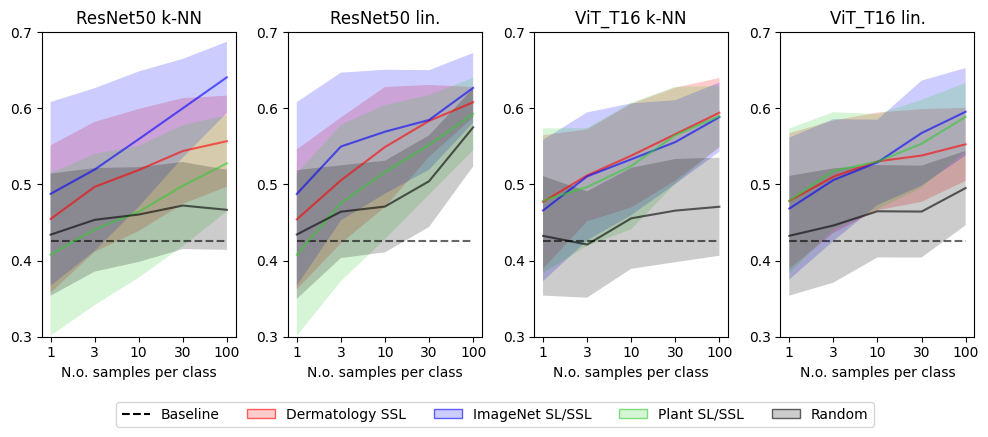
\includegraphics[width=15cm]{lines_ddi.png}
    \caption{Results of linear evaluation on subsampled sets from \gls{ddi}}\label{fig:lines_ddi}
    \end{center}
\end{figure}

\subsection{PAD-UFES-20}

\begin{figure}[H]
    \begin{center}
    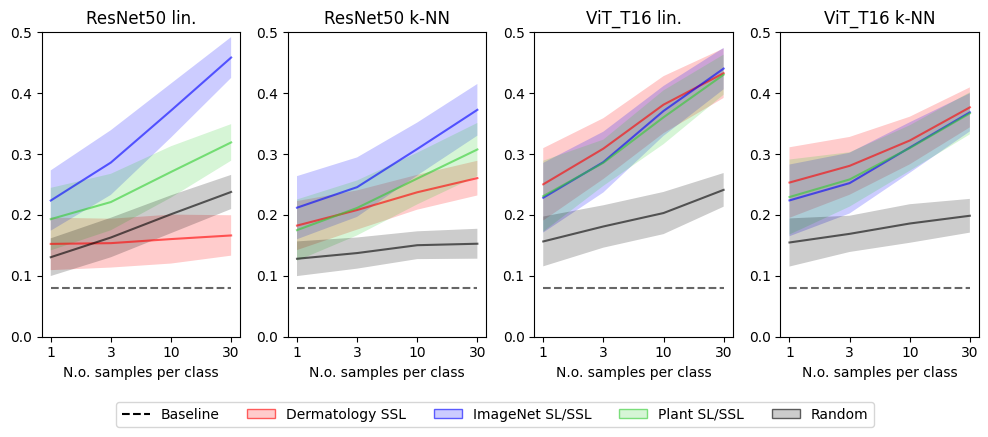
\includegraphics[width=15cm]{lines_pad-ufes-20.png}
    \caption{Results of linear evaluation on subsampled sets from PAD-UFES-20}\label{fig:lines_pad-ufes-20}
    \end{center}
\end{figure}

\subsection{HAM10000}

\begin{figure}[H]
    \begin{center}
    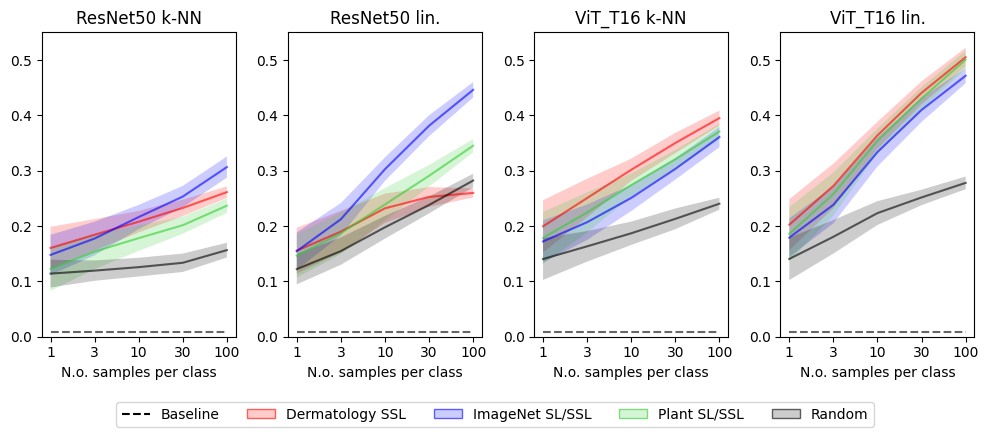
\includegraphics[width=15cm]{lines_ham10000.png}
    \caption{Results of linear evaluation on subsampled sets from HAM10000}\label{fig:lines_ham10000}
    \end{center}
\end{figure}

\subsection{Fitzpatrick17k}

\begin{figure}[H]
    \begin{center}
    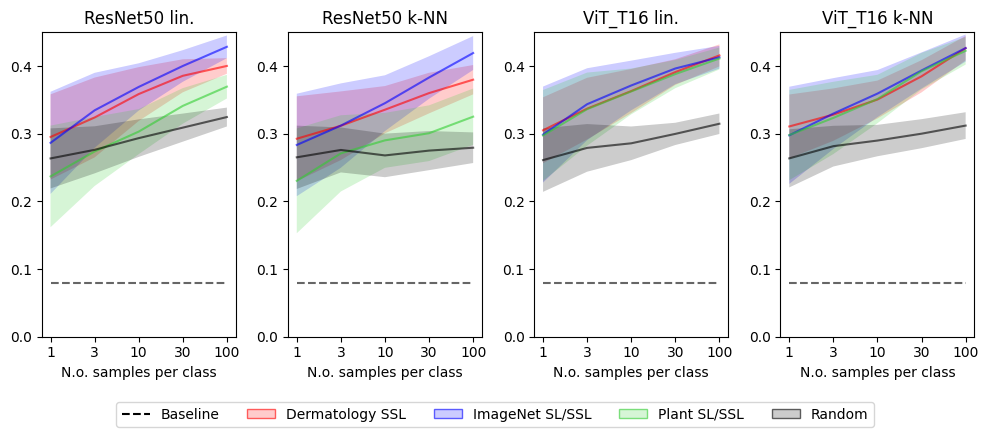
\includegraphics[width=15cm]{lines_fitzpatrick17k.png}
    \caption{Results of linear evaluation on subsampled sets from Fitzpatrick17k}\label{fig:lines_fitzpatrick17k}
    \end{center}
\end{figure}


% \section{Other}
% \subsection{DINO student/teacher}
% \subsection{Fine-tuning}
% \subsection{Fine-tuning}
